\thispagestyle{sectioned}
\chapter{Creative Commons Gadget}
%\addcontentsline{toc}{chapter}{\numberline{Creative Commons Gadget}}

The default license for any creation of any kind is the restrictive copyright. Copyright tries to ensure that all the rights remain to the original author of the content, but sometimes it can be advantageous to let people freely or semi-freely use, distribute or modify the content \cite{ref:oss_why}. \textbf{One of the most popular of these licenses}, with over 400 million \cite{ref:the_power_of_open} licensed works, are the Creative Commons set of licenses. These are not adecuate for licensing software, but in the context of Wave the content is usually creative text work, for which Creative Commons suits perfectly.

\label{subsec:cc_soa}
\section{State of the Art}
Wave doesnt have any way of publishing your content under any specific license. Kune has the option for publishing Waves in your personal space under one of the existing Creative Commons Licenses. Outside of the personal space, Kune preserves Wave's aspect and removes the space where the license is in the personal space, so no license is imposed to other participants in a wave.\\[.2cm]
Outside the world of wave, there's similar alternatives to the one trying to be implemented here. There is for example Creative Commons Configurator for Wordpress, which lets you set a license for your Wordpress posts. Creative commons also has a license chooser \cite{ref:cc_chooser} in their own webpage, that selects a license based on questions asked to learn the needs of the user.
\section{Results}
This extension allows participants to \textbf{set a Creative Commons license} to a specific blip, by inserting a gadget in the content and answering questions to reach the adequate license that meets the requierements. The Figure \ref{fig:cc_gadget} shows the final result of this extension.
\begin{figure}[h]
  \center
    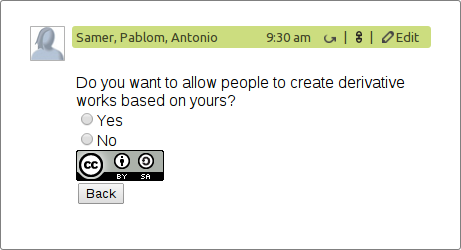
\includegraphics[keepaspectratio, scale=0.7]{Media/Captures/Extensions/CCGadget.png}
  \caption{Creative Commons Gadget}
  \label{fig:cc_gadget}
\end{figure}
Relating to the gadget structure described in Figure \ref{fig:gadget_classes}, this Gadget's Composite is the class CCGadgetMainPanel, the Messages relates to CCGadgetMessages and the GinModule would be represented by the class CCGadgetGinModule.\\[.2cm]
There is a limited amount of Creative Commons licenses, all of them requiring attribution of the original creator. There is some concepts which can be combined to build the different licenses:
\begin{itemize}
  \item Attribution: The used of this work has to be attributed to the original author and distributed with this attribution. If the BY is present, attribution is required.
  \item Derivation: Derivative works are those based on a previous work and modified to make a new work. If the ND is present, no derivated works are allowed.
  \item Commercial: A commercial work is that which seeks a profit directly or indirectly. If the NC is present, no commercial use of this work is allowed.
  \item Share Alike: Share the work the same way it was previously shared. If SA is present, usage of this work is forced to be shared alike.
\end{itemize}
Not all combinations of this concepts are possible, Table \ref{fig:cc_licenses} shows the existing licenses and their denominations.
\begin{table}[H]
  \begin{center}
    \begin{tabular}{ | l | c |}
      \hline
      CC-BY & Attribution\\
      CC-BY-ND & Attribution + No Derivatives\\      
      CC-BY-SA & Attribution + Share Alike\\
      CC-BY-NC & Attribution + Non Commercial\\
      CC-BY-NC-ND & Attribution + Non Commercial + No derivatives\\
      CC-BY-NC-SA & Attribution + Non Commercial + Share Alike\\
      \hline
    \end{tabular}
  \end{center}
  \caption{Available Creative Commons licenses}
  \label{fig:cc_licenses}
\end{table}
This gadgets keeps a variable for each one of this concepts and \textbf{asks a question to the user} to determine if the restriction has to happen or not, in order to figure out a valid license. The state stores the state of all the answers to the questions that can be asked, and the answers can be yes, no, or unanswered. When a question is answered a state delta is sent to the rest of the participants, and the image of the license is update to the best match from all the possible licenses. When all the answers are answered, only the image of the license remains linking to the whole chosen license.\\[.2cm]
\section{Conclusions and Future Work}
The main problem with this extension is the \textbf{limited amount of licenses}, only Creative Commons. Even though they are widely used, they might not cater to the tastes of everyone, or fit every possible position. There is also no way to license anything other than a blip, such as a blip and all its children or a whole wave.
\newpage
